\section{The geometry of depth in contract units}
\label{sec:depth}

\subsection{A marginal execution-price curve}

Fix a contract and a frozen list of eligible ordinary asks. At distinct prices $p_1<\cdots<p_k$, let available quantities be $q_1,\ldots,q_k$. Set $H_i=\sum_{j\le i}q_j$ and $H_0=0$. On the quantity interval $(0,H_k]$, define
\begin{equation}
 a(u)=p_i\quad\text{for }H_{i-1}<u\le H_i,
 \qquad K(Q)=m\int_0^Q a(u)\,du.
\label{eq:depth}
\end{equation}
For integer $Q$, this is the multiplier times the sum of the executed quote prices. Interpolation to real $Q$ is a mathematical device. It neither creates fractional contracts nor relaxes exchange lot constraints.

\begin{proposition}[Convex quote-value geometry]\label{prop:depth}
For $0\le Q\le H_k$, $K$ is continuous, piecewise linear, and convex. At an interior depth boundary $H_i$,
\begin{equation}
 \partial K(H_i)=[mp_i,mp_{i+1}],
 \qquad K''=m\sum_{i=1}^{k-1}(p_{i+1}-p_i)\delta_{H_i}
\end{equation}
in the distributional sense. The average execution price $K(Q)/(mQ)$ is nondecreasing for $Q>0$.
\end{proposition}
\begin{proof}
The derivative away from depth boundaries is $ma(Q)$, a nondecreasing step function. Its jumps are exactly $m(p_{i+1}-p_i)$, which establishes convexity, the subdifferential, and the distributional formula. Increasing $Q$ appends contracts whose prices are at least the average of the existing prefix. The average therefore cannot fall.
\end{proof}

No assumption that futures prices are positive is needed. If prices are negative, $K$ can decrease while remaining convex. What is increasing is the marginal price, not necessarily the level of the quote-value integral.

\subsection{Shortfall is a relative valuation}

Against benchmark price $p_0$, define buy execution shortfall
\begin{equation}
 \mathrm{IS}(Q;p_0)=K(Q)-mQp_0.
\label{eq:is}
\end{equation}
If all $Q$ purchased contracts remain open to a settlement $s$, their linear variation is
\begin{equation}
 \mathrm{VM}=mQs-K(Q)
 =mQ(s-p_0)-\mathrm{IS}(Q;p_0).
\label{eq:shortfallvm}
\end{equation}
Thus shortfall reduces the eventual marked gain by an exact dollar amount. It is not the initial margin deposit, and $K(Q)$ is not a bank debit at trade entry. Section~\ref{sec:settlement} gives the currency-rounded version and permits subsequent trades.

\begin{example}[An ES depth walk]\label{ex:depth}
Use ES asks of three contracts at 6,000.00, five at 6,000.25, and four at 6,000.50. A ten-contract buy fills $(3,5,2)$. With $m=50$,
\begin{align}
 K(10)&=50(3\cdot6000+5\cdot6000.25+2\cdot6000.50)\notag\\
      &=\$3{,}000{,}112.50,\\
 \bar p&=6000.225,\qquad
 \mathrm{IS}(10;6000)=\$112.50.
\end{align}
An average fill price need not itself lie on the order-entry grid. If the settlement is 6,001.00, the position receives \$387.50 in variation before fees: a \$500 benchmark gain less \$112.50 of execution shortfall.
\end{example}

\begin{figure}[htbp]
\centering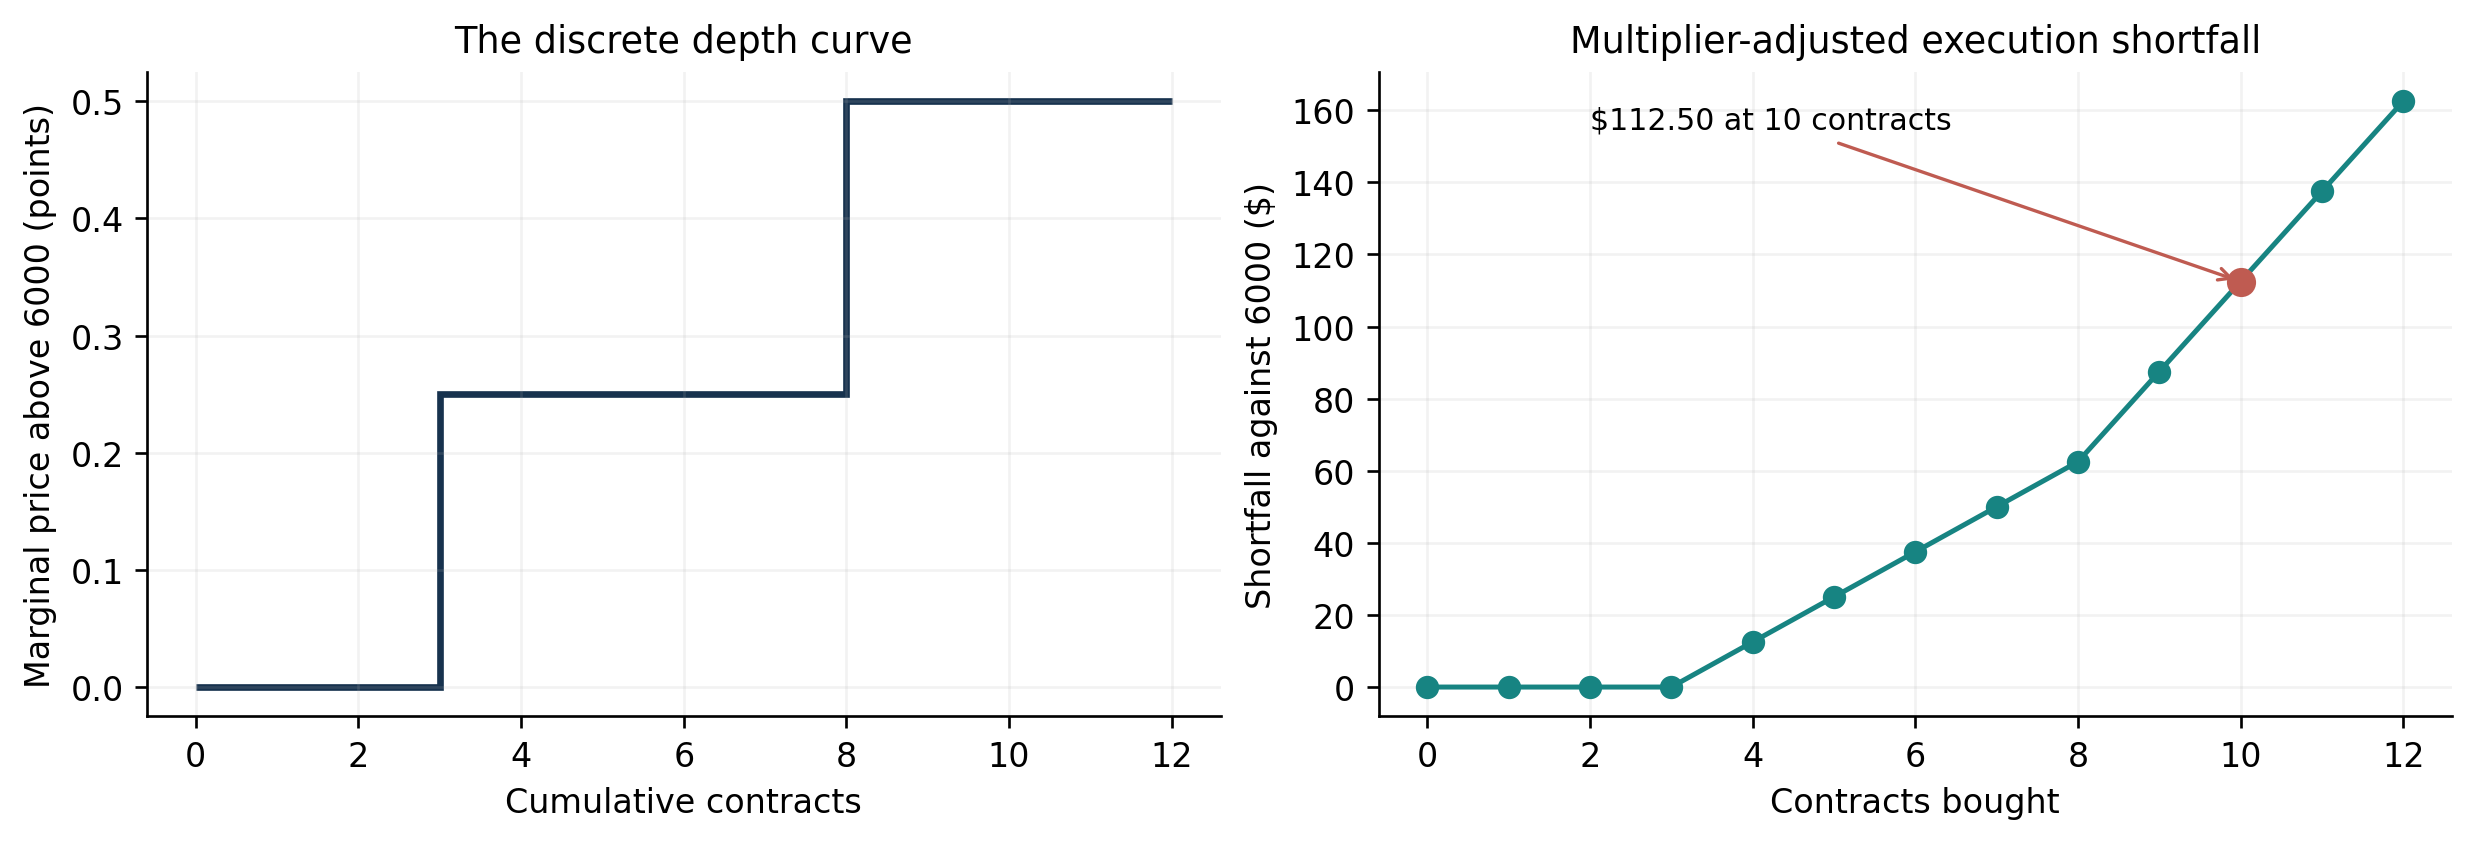
\includegraphics[width=\textwidth]{figures/02_depth.png}
\caption{The depth curve and execution shortfall in Example~\ref{ex:depth}. The slopes of the shortfall curve are the marginal price differences multiplied by \$50 per point.}
\label{fig:depth}
\end{figure}

\subsection{Price limits and perturbations}

\begin{corollary}[Buy-limit monotonicity]\label{cor:limit}
For a fixed quantity and a frozen ordinary book ranked first by price, increasing a buy limit cannot decrease the fill. If the original fill is positive, its average execution price weakly increases.
\end{corollary}
\begin{proof}
Newly eligible asks are appended after the original eligible list. Original fills are unchanged, and any additional contracts have prices at least as high as every originally eligible price. If no additional contracts fill, the average is unchanged; otherwise it is a weighted average of the original average and a weakly higher average.
\end{proof}

The assumptions exclude changes to implication, compatibility, and price controls during the match. With such changes, the eligible list itself must first be recomputed.

For two marginal curves $a,\widehat a$ on a common quantity interval,
\begin{equation}
 |K(Q)-\widehat K(Q)|
 \le m\int_0^Q|a(u)-\widehat a(u)|\,du.
\label{eq:depthbound}
\end{equation}
In particular a uniform price error $\delta$ yields a dollar error at most $mQ\delta$. This estimate exposes the importance of units: the same quote error has different financial consequences for contracts with different value factors. It also says nothing about queue priority, fill probability, or whether several implied quotes can be consumed simultaneously. Those are different parts of the state.
\FloatBarrier
